\chapter{(Ne)Reálne čísla}

\indexItem{Prg}{typy \vb{float} a \vb{double}}
Naše rozprávanie o základných typoch treba doplniť o ďalšie dva dôležité typy:
\prg!float! a \prg!double!. Slúžia na prásu s reálnymi (desatinnými) číslami.
V kapitole~\ref{sect:cisla} sme hovorili, že typy \prg!int!, \prg!long!, 
\prg!unsigned int!, \prg!char! a pod. ukladajú čísla v pamäti v dvojkovej
sústave vo fixnom počte bitov. Pri práci s desatinnými číslami je o jeden
problém naviac, a to, že idú donekonečna nielen smerom k veľkým číslam, ale
sú aj nekonečne husté. Keďže, podobne ako celočíselné typy, aj typy \prg!float!
a \prg!double! majú v pamäti rezervovaný fixný počet bitov (32, resp. 64), môže sa stať,
že dve veľmi blízke čísla sa zlejú do jedného. Aby sa šetrilo pamäťou, používa\indexItem{Mat}{vedecká notácia: mantisa a exponent}
sa tzv. vedecká notácia s {\em mantisou} a {\em exponentom}. Možno si niekedy videl
taký zápis v desiatkovej sústave, napr. $1.3\cdot10^5$, čo je $1.3\cdot100000=130000$.
Podobne $1.3\cdot10^{-5}=1.3\cdot0.00001=0.000013$. Je to veľmi príjemné, keď treba pracovať
s veľmi veľkými alebo veľmi malými číslami. V počítači je to podobné, iba
sa používa dvojková sústava. V dvojkovej sústave tiež môžeme používať ''desatinnú''
čiarku, napr. číslo $1011010.10011$ v dvojkovej sústave je


\centerline{\begin{tikzpicture}
  \foreach \v/\p [count=\i] in { 1/64, 0/32, 1/16, 1/8, 0/4, 1/2, 0/1, 
  1/{\frac{1}{2}}, 0/{\frac{1}{4}}, 0/{\frac{1}{8}}, 1/{\frac{1}{16}}, 1/{\frac{1}{32}}  } {
    \draw[dotted, shorten <= 2ex, shorten >= 2ex] 
    (\i,0) node [color=green!70!black] {{\small $\p$}}
     -- (\i,-6ex) node {\v};
  }
\end{tikzpicture}}


$64+16+8+2+0.5+0.0625+0.03125=90.59375$ v desiatkovej. Pre zapamätanie čísel
sa tieto najprv normalizujú tak, aby ''desatinná'' čiarka bola hneď za prvou jednotkou.
Naše číslo $90.59375$ by sme preto v dvojkovej sústave zapísali $1.01101010011\cdot2^6$.
Časť \vb{01101010011} sa volá mantisa a \vb{6} je exponent. Typ \prg!float!
má vyhradený jeden bit na znamienko, 8 bitov na exponent a 23 bitov na mantisu. 
K hodnote exponentu sa priráta 127, aby sme mohli mať aj záporné exponenty a
nemuseli ukladať zvlášť znamienko.
Naše číslo by preto v pamäti vyzeralo takto (exponent je $127+6=133$, čo je v 
dvojkovej sústave \vb{10000101}):


\centerline{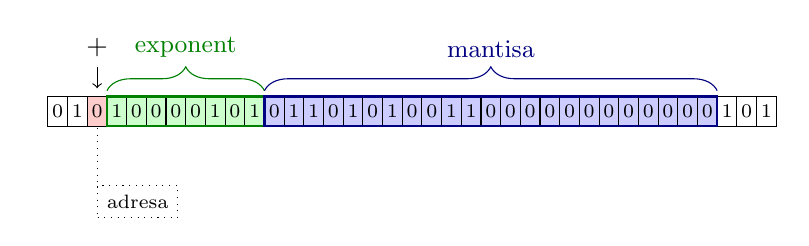
\begin{tikzpicture}[scale=0.25]
  \def\var#1#2#3#4{%
    \draw[#4] decorate[
       decoration={brace, amplitude=2ex}]{
       (#1,1.8) -- (#1+#2,1.8) node [align=center,midway,anchor=south,yshift=2ex] {\vb{#3}}
        };
   \draw[#4,thick] (#1,0) rectangle (#1+#2,1.5);

  }

  \filldraw[draw=none,fill=red!20!white](3,0) rectangle (4,1.5); 
  \filldraw[draw=none,fill=green!20!white](4,0) rectangle (12,1.5); 
  \filldraw[draw=none,fill=blue!20!white](12,0) rectangle (35,1.5); 

  \foreach \v [count=\i] in { 0,1, 
    0,  1,0,0,0,0,1,0,1,  0,1,1,0,1,0,1,0,0,1,1,0,0,0,0,0,0,0,0,0,0,0,0,    1,0,1
  }{
    \draw (\i,0) rectangle node [anchor=center] {{\scriptsize\roboto \v}} (\i+1,1.5);
  }

  \draw [->, shorten >= 3] (3.5,3) node[anchor=south]{$+$} -- (3.5,1.5);
  
  \var48{{\small exponent}}{green!50!black}
  \var{12}{23}{{\small mantisa}}{blue!50!black}

  \draw[dotted] (3.5,-0.1) -- (3.5,-3) 
  node[draw, anchor = north west]{\scriptsize adresa};

\end{tikzpicture}}

\indexItem{Prg}{typ float}
 Drobné technické detaily som zamlčal, ale pre nás to teraz stačí. To, čo je dôležité 
vedieť je, že v premennej typu \prg!float! síce môžeme mať zapamätané aj veľmi veľké
čísla, ale potom nemáme veľkú presnosť. Skús si napríklad takýto program:


\vbox{
\begin{lstlisting}[] 
#include <iostream>
using namespace std;

int main() {
  float a, b;
  cin >> a;
  b = a + 1;
  cout << fixed << a << endl;
  cout << b << endl;
  if (a == b) cout << "rovnake" << endl;
  else cout << "rozne" << endl;
}
\end{lstlisting}
}

\indexItem{Prg}{\vb{fixed}}
 (\vb{fixed} je, podobne ako \vb{endl}, špeciálna hodnota, ktorá spôsobí, 
že \prg!cout <<! nebude používať vedeckú notáciu). Keď program spustíš a na vstupe 
napíšeš \vb{12.3}, vypíše sa, presne ako očakávaš, 

\begin{outputBox}
12.300000
13.300000
rozne
\end{outputBox}

Ale keď na vstupe zadáš \vb{16777216} (čo je $2^{24}$),
vypíše sa

\begin{outputBox}
16777216.000000
16777216.000000
rovnake
\end{outputBox}

Čo sa stalo? Vstupné (celé) číslo je v dvojkovej sústave jednotka a za ňou
24 núl, zapamätá sa teda ako $1.0\ldots0\cdot2^{24}$, čiže má
exponent $151$ ($127+24$)  a mantisu $0$. Potom k nemu prirátaš 1 a dostaneš
číslo, ktoré má jednotku, potom 23 núl a potom zase jednotku. Opäť by teda exponent
bol $151$, ale mantisa nemá dosť miest -- prvých 23 miest mantisy sú muly a jednotka
na 24tom mieste sa stratí. Na podobné efekty si treba dávať pozor, môžu okrem iného
spôsobiť, že výsledok niekoľkých operácií môže stratiť presnosť a test na rovnosť
dvoch \prg!float! čísel je vždy ošemetný. Pri type \prg!double!, ktorý má 64 bitov
(exponent 11 bitov a mantisa 52 bitov) sú efekty straty presnosti menej viditeľné,
ale tiež ich treba  mať na pamäti. Posledná vec: konverzia \prg!(int)a!, kde \vb{a}
je typu \prg!float! alebo \prg!double! vráti odrezanú desatinnú časť (t.j.
\prg!(int)12.3! je \vb{12} a \prg!(int)-12.3! je \vb{-12}). Ak sa výsledné číslo
nezmestí do \prg!int!, hodnota môže pretiecť, napr. ak máš
\prg!float a = 4294967297.0;! tak \prg!cout<<(int)a;! vypíše \vb{-2147483648} (čo je
$-2^{31}$)a \prg!cout << (unsigned int)a;! vypíše \vb{0}.

